\section{\K 串联谐振电路}
\subsection{\K 串联谐振的原理}
\Par 一般而言,RLC串联电路中的总电流和总电压通常是不同相位的,但是在某一特定的电源频率下,$u$和$i$可以达到同相位,此时电路呈电阻性,我们称电路在该频率下发生了\textbf{谐振}.

\Par 我们知道
\begin{equation*}
    \frac{\dot{U}}{\dot{I}}=\left[ R+\mathrm{j}\left( X_{\mathrm{L}}-X_{\mathrm{C}} \right) \right] 
\end{equation*}
要想电路呈电阻性,就是让阻抗角$\varphi =0$,也就是虚部为0,因此电路发生谐振的条件为
\begin{equation}
    \frac{\dot{U}}{\dot{I}}=\left[ R+\mathrm{j}\left( \omega L-\frac{1}{\omega C} \right) \right] \Rightarrow \omega L-\frac{1}{\omega C}=0\Rightarrow \omega =\frac{1}{\sqrt{LC}}=\omega _0
\end{equation}
其中,$\omega$为激励频率,$\omega _0$为电路的固有频率.同时我们也可以写成频率的形式
\begin{equation}
    f=\frac{1}{2\pi \sqrt{LC}}
\end{equation}

\begin{wrapfigure}{r}{0.25\textwidth}
    \centering
    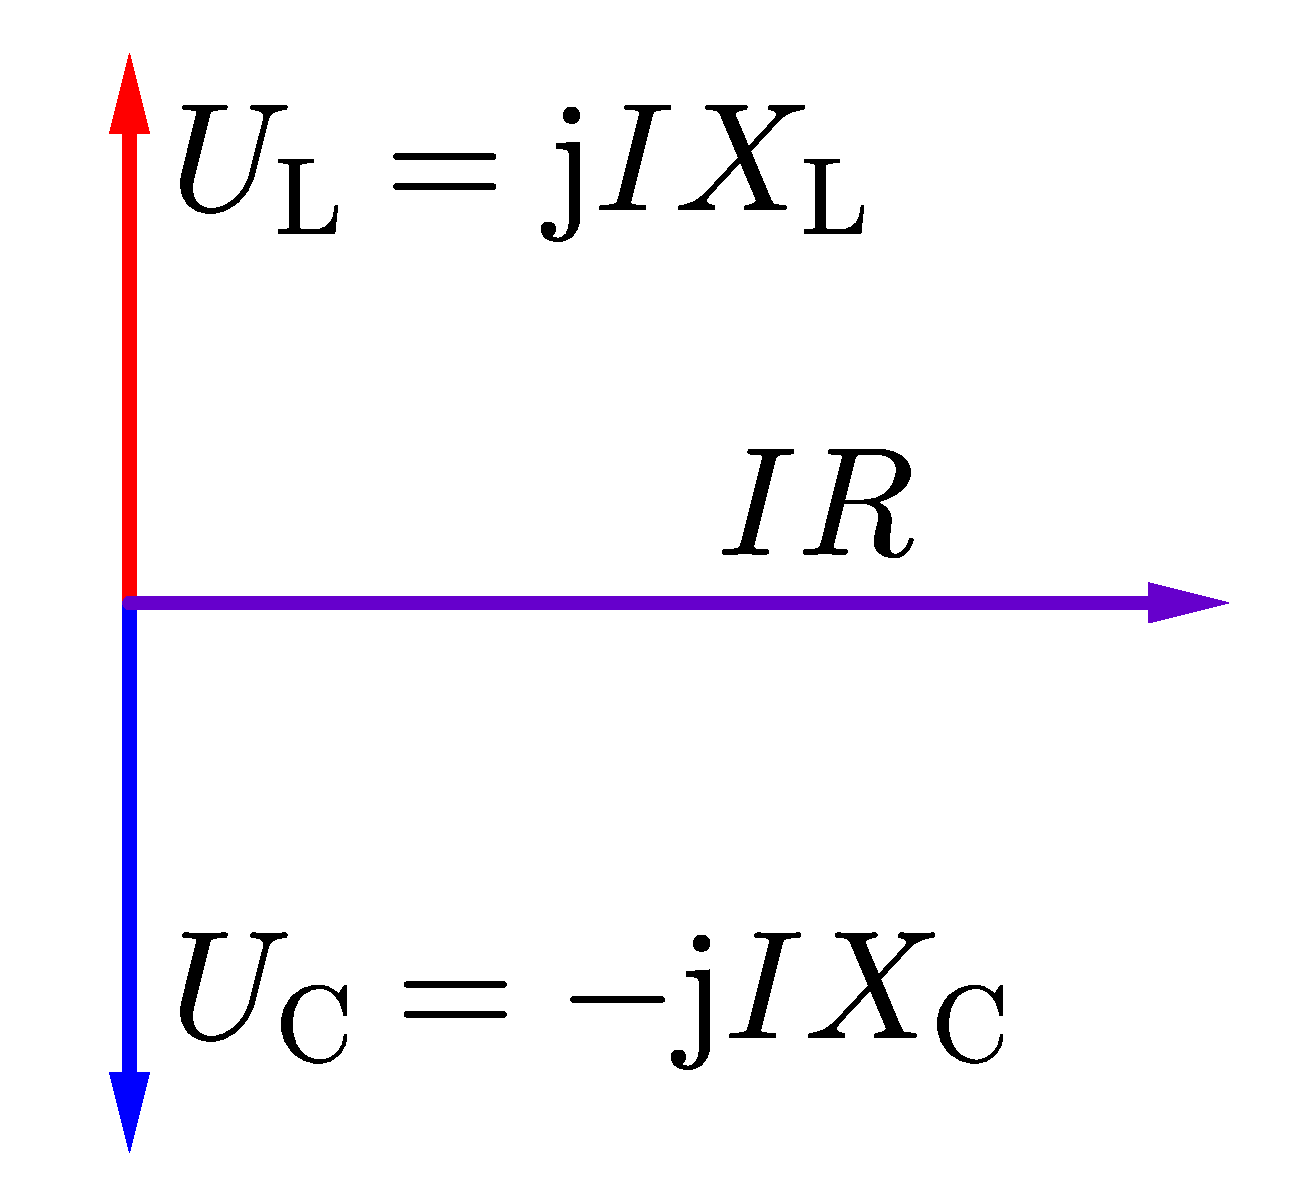
\includegraphics[width=0.25\textwidth]{谐振电压.pdf}
    \caption{谐振电压}
    \label{fig:谐振电压}
\end{wrapfigure}
\Par 阻抗模的表达式为
\begin{equation}
    \left| Z \right|=\sqrt{R^2+\left( \omega L-\frac{1}{\omega C} \right) ^2}
\end{equation}
当电路谐振时,阻抗模$\left| Z \right|$取到最小值.

\Par 由
\begin{equation}
    I=\frac{U}{\left| Z \right|}
\end{equation}
可以知道,当电路谐振时,电流大小取到最大值.

\Par 我们画出串联电路的相量图\ref{fig:谐振电压},可以知道此时
\begin{equation*}
    \omega L=\frac{1}{\omega C}
\end{equation*}
因此电感分压与电容分压互相抵消,电路电压等于电阻电压.

\subsection{\K 串联谐振的应用}

\begin{wrapfigure}[6]{r}{0.2\textwidth}
    \centering
    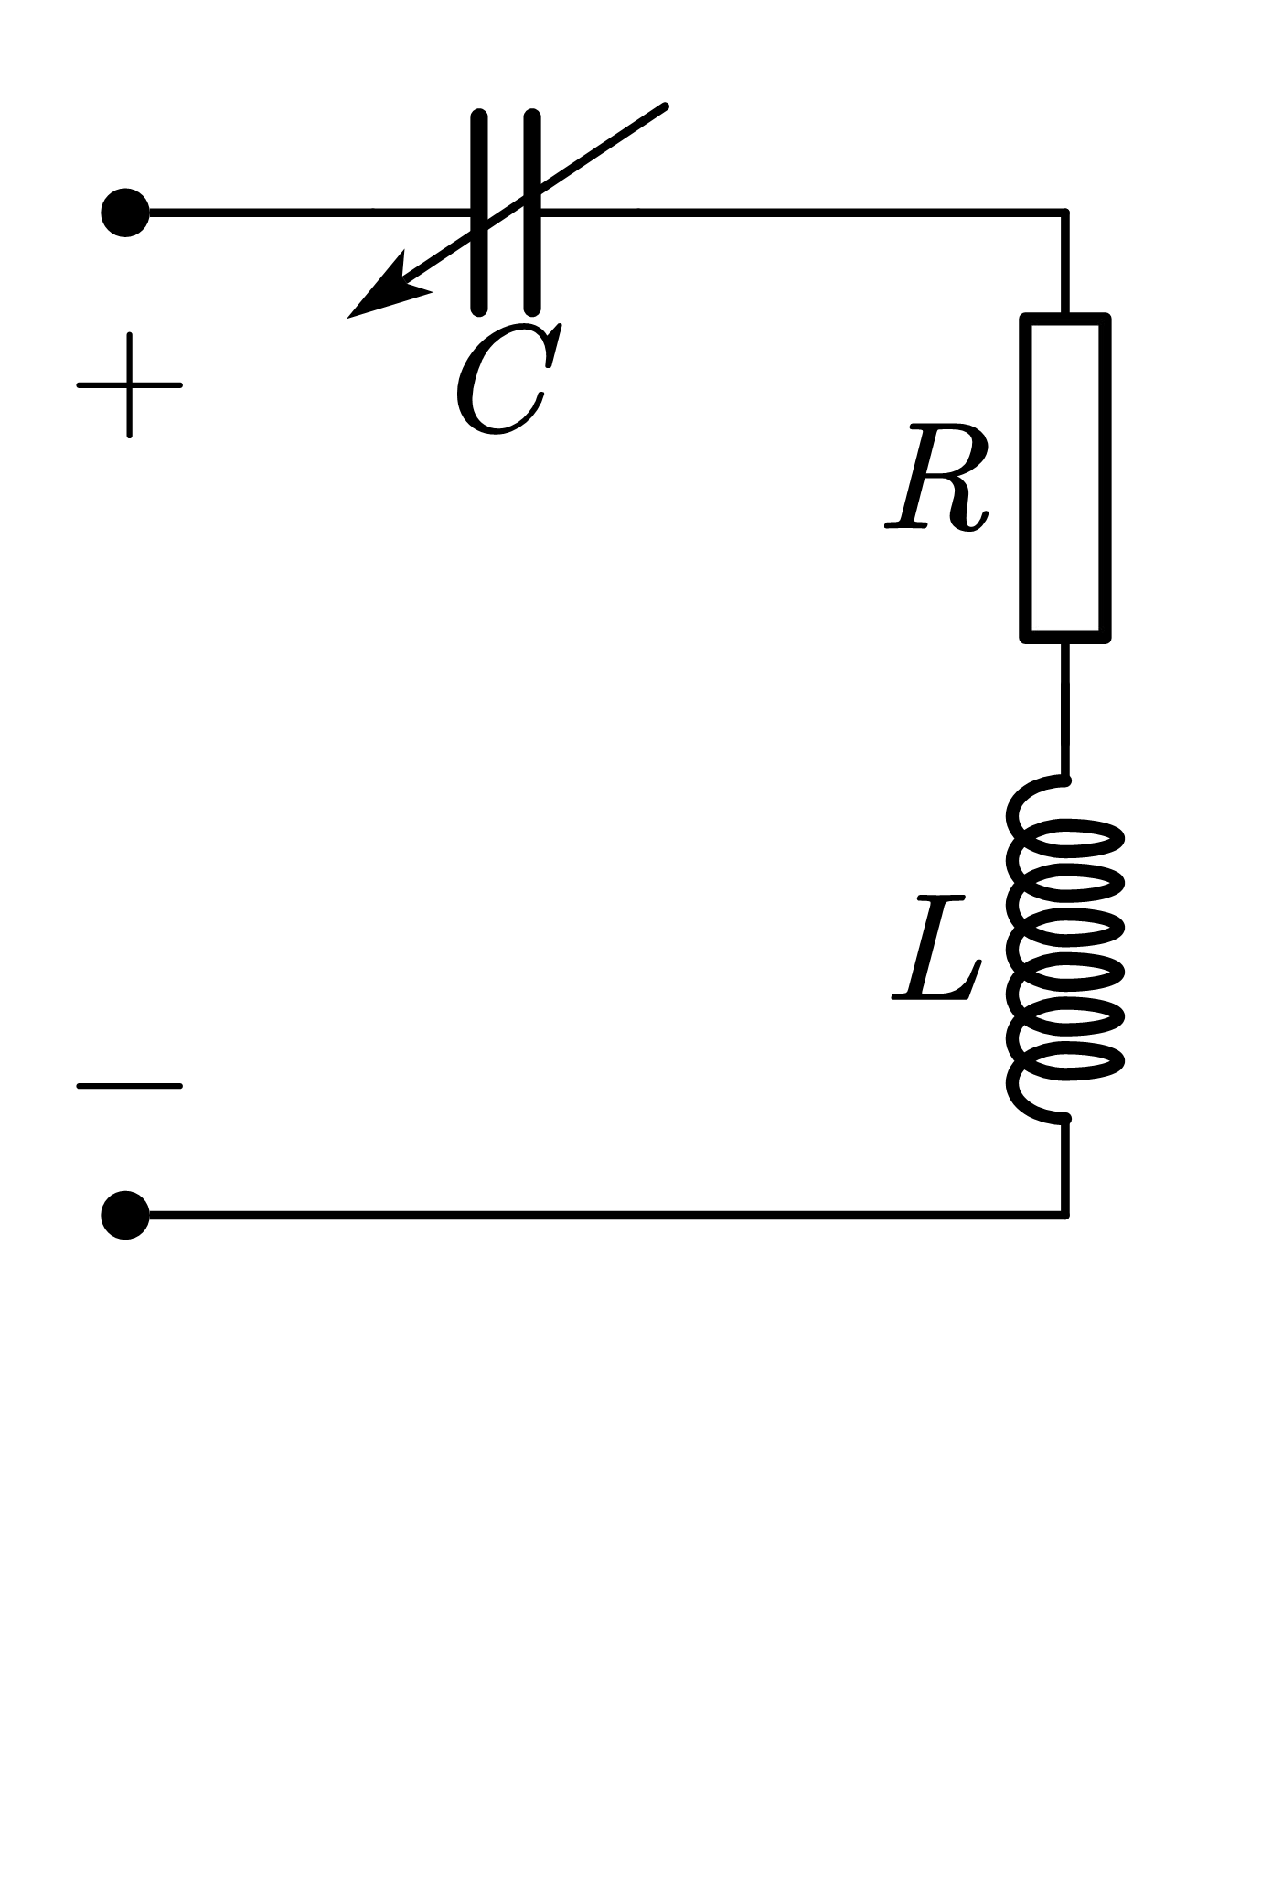
\includegraphics[width=0.2\textwidth]{收音机.pdf}
    \caption{收音机}
    \label{fig:收音机}
\end{wrapfigure}
\begin{example}
    收音机的电路如图\ref{fig:收音机}所示,只有处于谐振频率的电台信号能够以最大能量有效地向后方电路传递,其他的电台信号均被抑制或筛除,这就是收音机调频的原理.
    
    \Par 在该电路中,$L=250\mathrm{\mu H}$,$R=20\Omega $,现在可以用可调电容调整电路的固有频率.试问:若市电台的频率为$f=820\mathrm{KHz}$,想要接收到市电台的广播,应当把可调电容的容值调整为多少?
\end{example}
\begin{solution}
    根据
    \begin{equation}
        f=\frac{1}{2\pi \sqrt{LC}}
    \end{equation}
    我们可以知道
    \begin{equation}
        C=\frac{1}{\left( 2\pi f \right) ^2L}\approx 150\mathrm{pF}
    \end{equation}
\end{solution}
\Par 对于这个例题,我们提出疑问,谐振频率的电台信号究竟被放大了多少呢?而其他的电台信号有被抑制了多少呢?

\Par 现在有三个电台频率和它们的谐振电容容值
\begin{equation*}
    \begin{aligned}
        f_{\text{省}}&=640\mathrm{KHz}\\
        f_{\text{市}}&=820\mathrm{KHz}\\
        f_{\text{县}}&=1026\mathrm{KHz}\\
    \end{aligned}\Longrightarrow \begin{aligned}
        C_{\text{省}}&=248\mathrm{pF}\\
        C_{\text{市}}&=150\mathrm{pF}\\
        C_{\text{县}}&=96\mathrm{pF}\\
    \end{aligned}
\end{equation*}
设三个电台在收音机上产生的感应电动势为$E_1=E_2=E_3=10\mathrm{\mu V}$,我们可以求得
\begin{table}[htbp]
    \centering
    \begin{tblr}{
        row{odd} = {azure8}, 
        row{even} = {gray8},
        colspec={cccc},
        row{1} = {c,2em,azure2,fg=white}
        }
        序号    & 电台频率  & 阻抗($X=X_{\mathrm{L}}-X_{\mathrm{C}}$) & 电流\\
        省电台  & $640\mathrm{KHz}$ & $X=1000-1660=-660\Omega $  & $I=\frac{U}{\left| X \right|}\approx 0.015\mathrm{\mu A}$\\
        市电台  & $820\mathrm{KHz}$ & $X=1290-1290=0\Omega $     & $I=\frac{U}{\left| X \right|}\approx 500\mathrm{\mu A}$\\
        县电台  & $1026\mathrm{KHz}$& $X=1612-1034=578\Omega $   & $I=\frac{U}{\left| X \right|}\approx 0.017\mathrm{\mu A}$\\
    \end{tblr}
\end{table}

\Par 我们定义:在谐振频率下,电容或电感的分压与路端电压的比值
\begin{equation}
    Q=\frac{U_{\mathrm{L}}}{U}=\frac{U_{\mathrm{C}}}{U}
\end{equation}
被称作\hl{品质因数}.品质因数$Q$越大,该电路对特定频率信号的选择性就越好.这样一个电路中,它的品质因数$Q=64.5$,如果将电感的感值减半,电容的容值倍增,新电路的品质因数$Q'=32.3$,如果再一次将电感的感值减半,电容的容值倍增,新电路的品质因数$Q''=8.1$.








